\chapter{Keeping Serverless Computing Alive with Greedy-Dual Caching}
\label{chap:faascache}

% \todo{FaasCache Intro paragraph}
Keeping every created function container indefinitely is not feasible for serverless control planes.
They can be invoked sparsely -- perhaps a handful of times per day.
When a container isn't handling an invocation, it sits idle, occupying memory the control plane may want to use for other, more active, purposes.
How long to keep a function sandbox in memory is called a \textbf{keep-alive} decision, and has a dramatic effect on latency.

The primary goal of keep-alive is to amortize the initialization and cold start latencies by keeping functions alive for different durations based on their characteristics.
Keep-alive policies must be generalizable and yield high server utilization, because servers must handle hundreds of short-lived functions concurrently.
Functions can have vastly different characteristics, and keep-alive policies must work efficiently in highly dynamic and diverse settings.
We use the following characteristics of functions for keep-alive policies.

The \textbf{initialization time} of functions can vary based on the code and data dependencies of the function.  
For example, a function for machine learning inference may be initialized by importing large ML libraries (such as TensorFlow, etc.), and fetching the ML model, which can be hundreds of megabytes in size and take several seconds to download. 
Functions also differ in terms of their \textbf{total running time}, which includes the initialization time and the actual execution time. 
Again, functions for deep-learning inference can take several seconds, whereas functions for HTTP servers and microservices are extremely short-lived (few milliseconds). 
The \textbf{resource footprint} comprises the CPU, memory, and I/O use, and also differs widely based on the application's requirements. 
Finally, functions have different \textbf{frequencies} and invocation rates. Some functions may be invoked several times a second, whereas other functions may only be invoked rarely (if they are used to serve a very low-traffic website, for instance). 


\subsection{Caching Background}

% This whole thing needs to be rewritten. What is the message?

% This is nice, but here and not in the technical sections? 
Our answer to solving the twin conundrum of keep-alive and provisioning that is robust to workload heterogeneity and dynamism, is to use concepts from a related, well-known field with the same challenges. 
%
Caching has a long history of robust eviction algorithms that use temporal locality such as  LRU (Least Recently Used). 
The effectiveness of a caching algorithm depends on the workload's inter arrival time distribution, the relative popularities of different objects, and thus many variants of LRU such as LRU-k~\cite{o1993lru}, segmented LRU~\cite{cheng2000lru}, ARC~\cite{megiddo2003arc}, and frequency based eviction such as LFU~\cite{einziger2017tinylfu}, are widely used in caching systems. 
Because functions show a lot of diversity in their memory footprints, and since keep-alive is primarily constrained by server memory, we seek to use \emph{size-aware} caching methods. 
%Conventional caching \emph{largely} deals with constant-sized objects. For example: LRU, sampling techniques like SHARDS, counterstacks, etc.
%Therefore, we investigate the use of \emph{size-aware} techniques for keep-alive policies and provisioning.
While conventional caching algorithms and analytical models largely deal with constant-sized objects, many size-aware caching policies have been developed for web-pages and data~\cite{cao_irani_1997}. 
In particular, we use the Greedy-Dual~\cite{young_gd_orig_94} online caching framework that deals with objects with different eviction costs, that are determined based on size and other factors.
The Greedy-Dual family of eviction algorithms for non-identical objects can be extended in many ways.
We use a common variant, Greedy-Dual-Size-Frequency~\cite{gdsf, gdfs_2001,cherkasova2001role}, which considers the size and frequency of objects. 


Caching has a rich collection of analytical and modeling techniques to determine the efficacy of caches for different workloads.
%Analysis techniques such as stack distances help in cache provisioning, are based on hit-ratio curves, and provide the fraction of accesses which are cache-hits for different cache sizes.
Hit (or miss) ratio curves are widely used for cache sizing to achieve a target performance, and for understanding and modeling cache performance. 
Hit-ratio curves can be constructed both in an offline and online manner, using techniques involving reuse distances~\cite{osca_atc20}, eviction times~\cite{hu2016kinetic}, Che's approximation~\cite{che2002hierarchical}, footprint descriptors~\cite{sundarrajan2017footprint}, and estimation techniques such as SHARDS~\cite{shards}, counterstacks~\cite{counterstacks}, etc. 



\section{Keep-alive Tradeoffs}
\label{sec:tradeoffs}


In this section, we first present an empirical analysis of cold-start overheads of common serverless applications, followed by the tradeoffs in keep-alive policies. 

\noindent \textbf{System model.} 
We assume that each function invocation runs in its own container. 
%
A FaaS control plane may use a cluster of physical servers, and forward the function invocation requests to different servers based on some load-balancing policy. 
Our aim is to investigate general techniques that are independent of cluster-level load-balancing, and we therefore focus on \emph{server-level} policies. 
Even on a single server, a function can have multiple independent and concurrent invocations, and hence containers. 
Each function has its own container disk-image and initialization code, and thus containers cannot be used by different functions. 
A function's containers are nearly identical in their initialization overheads and resource utilization, since they are typically running the same function code. 
%
When a function finishes execution, its container may be terminated, or be kept alive and ``warm'' for any future invocations of the same function. 
%
At any instant of time, each container is either running a function, or is being kept alive/warm. % (see Figure~\ref{fig:server}). 
%
Thus, server resources are consumed by running containers, and containers being kept alive in anticipation for future invocations. 


%rev1 
Keeping functions alive/warm presents a fundamental tradeoff: it can reduce application-latency and CPU and I/O overhead, but it increases memory pressure. 
Nevertheless, recycling the execution environment and keeping function containers alive is a useful performance optimization that is supported by large public cloud platforms~\cite{goog-functions-tricks,aws-warm-predictable,azure-warmup-trigger}. 
%
In some scenarios, server resources may also be shared with long-running containers and VMs. 
In such cases, function keep-alive also influences the performance of other co-located applications and services, and the overall cloud efficiency. 
Therefore, understanding and optimizing this tradeoff is important, and we develop caching-based dynamic resource provisioning policies in Section~\ref{sec:provision}. 
Our goal is to allow FaaS operators to understand the benefits of different levels of aggressive keep-alive policies. 


\noindent \textbf{Cold-start overheads in OpenWhisk.} 
%
In order to understand the performance and latency implications of function cold-starts, we investigate the chain of events necessary to run function code in a popular FaaS control plane, OpenWhisk~\cite{openwhisk}.  
A timeline of a function invocation request for a TensorFlow machine learning inference task is shown in Figure~\ref{fig:timeline}. 
The figure shows the major sources of cold-start overhead: from request arrival to the actual function execution. 
OpenWhisk first checks whether the function can be served from the  pool of warmed containers it maintains, and if no container is found, a Docker container is launched, and the runtime for the function is initialized: which comprises of OpenWhisk and Python runtime initialization, as well as any specific \emph{explicit} function initialization provided by the application. 
The total compulsory overhead, from the request arrival to the actual function execution, is significant: up to 2.5 seconds are spent loading all runtime dependencies, before the user-provided initialization and actual event handling code can begin execution. 


\begin{figure}[t]
  \centering
  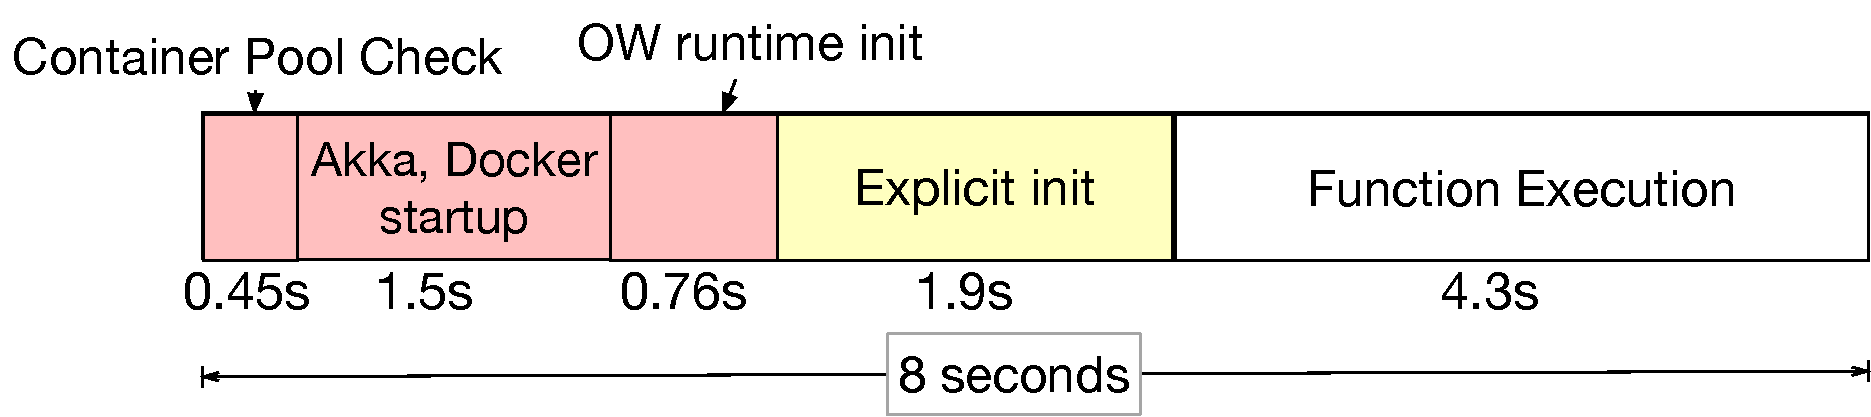
\includegraphics[width=0.8\textwidth]{faascache/faas-keepalive-20/figures/ow-timeline.pdf}
  \caption{Timeline of function execution and sources of cold-start delay in OpenWhisk for an ML inference application.}
  \label{fig:timeline}
\end{figure}


\noindent \textbf{Function Initialization.}
%\noindent \textbf{Function Initialization.}
%
%Optionally, applications may also use custom code to initialize and pre-warm the container 
%rev1 first and last line 
%Explicit
Function initialization refers to function-specific code for downloading and resolving code and data dependencies, which can be run before actual function execution (explicit-init component in Figure~\ref{fig:timeline}). 
For example, this can be used for downloading data dependencies ahead of time such as large neural network models for inference, or for runtime initialization such as downloading and importing package dependencies (e.g., Python packages). 
%The second technique for reducing the cold-start overhead is to explicitly initialize functions before running  them, and resolving most of the function's code and data dependencies during the initialization phase. 
%
An example of function initialization is shown in Figure~\ref{fig:lambda-example}, which shows a pseudo-code snippet of a function that performs machine learning inference on its input. 
For ML inference, the function downloads an ML model and initializes the TensorFlow ML framework (lines  5 and 6). 
If the function's container is kept alive, then invocations of the function do not need to run the expensive initialization code (lines 2--6). 
%Thus, the execution latency of functions can be minimized with a combination of careful function initialization and keeping the containers alive. 
% too broad a conclusion here...


% \footnotesize
\begin{figure}
\begin{lstlisting}[language=Python, numbers=left, frame=single, basicstyle=\footnotesize\sffamily, columns=fullflexible, xleftmargin=10.0ex, xrightmargin=10.0ex]
#Initialization code 
import numpy as np 
import tensorflow as tf
  
m = download_model('http://model_serve/img_classify.pb')
session = create_tensorflow_graph(m) 
  
def lambda_handler(event, context):
     #This is called on every function invocation 
     picture = event['data']
     prediction_output = run_inference_on_image(picture) 
     return prediction_output 
   \end{lstlisting}
   %\vspace*{\myfigspace}
   \caption{Initializing functions by importing and downloading code and data dependencies can reduce function latency by hiding the cold-start overhead.}
   \label{fig:lambda-example}
   %\vspace*{\myfigspace}
\end{figure}


% The function cold-start overhead includes both the execution environment initialization and the
\begin{comment}
Explicit initialization allows functions to be pre-warmed, and can be used to reduce the cold-start overhead. 
However, explicit initialization is not common---our empirical investigation into FaaS benchmarks~\cite{kim_functionbench_2019} and official examples showed that applications do not use this functionality. 
Nevertheless, it can be a powerful technique to amortize expensive operations such as package imports and downloading data dependencies. 
Explicit initialization can thus increase the effectiveness of keep-alive. 
However because it is not ubiquitous, we assume it is \emph{optional}, and our keep-alive and provisioning techniques work with and without it. 
\end{comment}


\noindent \textbf{Workload Diversity and Dynamism.}
%
Designing keep-alive policies is not trivial due to the highly diverse and expanding range of applications that are using FaaS control planes.
%This is in tradeoffs category. 
Conventionally, FaaS has been used for hosting web services, which is attractive because of the pay-per-use properties. 
Event handling functions for web responses typically have a small memory footprint but require low execution latency. 
Increasingly, FaaS is also being used for ``heavy'' workloads with high memory footprint and large initialization overheads such as highly parallel numerical computing (such as matrix operations~\cite{jonas2017occupy}, scientific computing~\cite{shankar2018numpywren}, and machine learning~\cite{akkus_sand_2018}. 
The diversity of FaaS applications also results in a wide range of function memory footprints, running times, and initialization times, as seen in Table~\ref{tab:workloads}.  
Keep-alive policies must therefore balance the resource footprint of the containers with the benefits of keeping containers alive---and do so in manner that is applicable across a wide range of applications. 


Furthermore, FaaS workloads show a high degree of dynamism and temporal effects. 
The Azure function~\cite{shahrad_serverless_2020} trace shows sharp diurnal effects: the function arrival rate is about $2\times$ higher during the peak periods compared to the average. 
Function workloads are also heavy-tailed: a few ``heavy hitting'' functions are invoked much more frequently than others or consume a larger amount of computing resources, often by 2 or 3 orders of magnitude. 


\subsection{Policy Goals and Considerations}


The primary goal of keep-alive is to reduce the initialization and cold-start latency, by keeping functions alive for different durations based on their characteristics. 
% Servers that run these functions are heavily multiplexed, and run hundreds of short lived functions concurrently. %backend FaaS servers?
% too sudden 
Because servers run hundreds of short lived functions concurrently, keep-alive policies must be generalizable and yield high server utilization. 
Functions can have vastly different characteristics, and keep-alive polices must work efficiently in highly dynamic and diverse settings. % (Table~\ref{tab:workloads}). 
We use the following characteristics of functions for keep-alive policies.


The \textbf{initialization time} of functions can vary based on the code and data dependencies of the function.  
For example, a function for machine learning inference may be initialized by importing large ML libraries (such as TensorFlow, etc.), and fetching the ML model, which can be hundreds of megabytes in size and take several seconds to download. 
Functions also differ in terms of their \textbf{total running time}, which includes the initialization time and the actual execution time. 
Again, functions for deep-learning inference can take several seconds, whereas functions for HTTP servers and microservices are extremely short-lived (few milliseconds). 
The \textbf{resource footprint} comprises of the CPU, memory, and I/O use, and also differs widely based on the application's requirements. 
Finally, functions have different \textbf{frequencies} and invocation rates. Some functions may be invoked several times a second, whereas other functions may only be invoked rarely (if they are used to serve a very low-traffic web-site, for instance). 

% \begin{figure}[t]
%   \centering
%   \vspace*{\myfigspace}
%   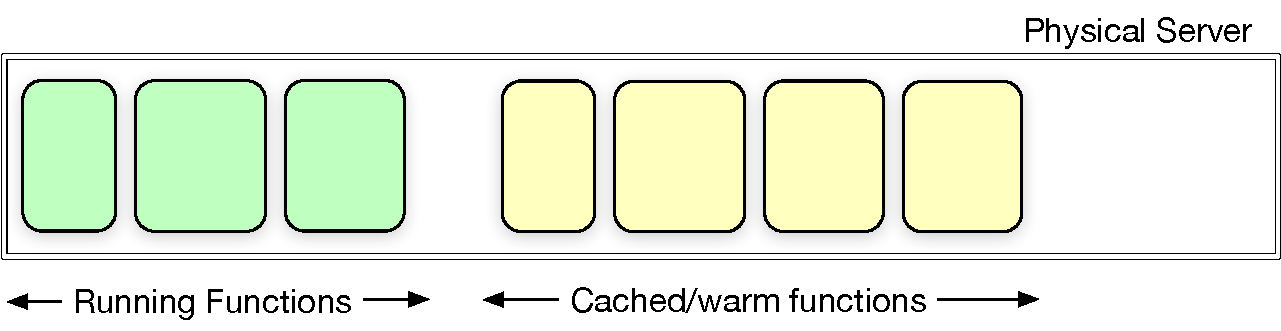
\includegraphics[width=0.4\textwidth]{../graphs/faas.pdf}
%   \vspace*{\myfigspace}
%   \label{fig:runwarm}
%   \caption{Server resources are consumed by running and warm containers.}
%     \vspace*{\myfigspace}
% \end{figure}


Because server resources are finite, it is important to prioritize functions which should be kept alive, based on the aforementioned characteristics. 
A function which is not popular and is unlikely to be called again in the near future, sees little benefits from keep-alive, and wastes server memory. 
%In fact, keeping such functions alive consumes valuable server computing resources for no gain in efficiency. %energy.. hmm
%Thus, keep-alive policies should prioritize popular functions. 
Similarly, the resource consumption of the functions is also important: since keeping large-footprint functions alive is more expensive than smaller functions, smaller functions should be preferred and kept alive for longer. 
Finally, functions can also be prioritized based on their initialization overhead, since it is effectively wasted computation.

% This paragraph is key. Different priorities and there is no one single ranking scheme for keepalive... 
The problem of designing keep-alive policies is complicated by the fact that functions may have vastly different keep-alive priorities for the different characteristics.
Consider a function with a large memory footprint (like those used in ML inference), high initialization overhead, and a low popularity.
Such a function should have a low keep-alive priority due to its size, high priority due to large initialization overhead, and a low priority due to its low popularity.
Thus, keep-alive policies must carefully balance all the different function characteristics and prioritize them in a coherent manner. 


% This still reads like making a case. But its only two sentences and bears repeating?
Current FaaS systems have shirked from this challenge and use primitive keep-alive policies that are not designed with the diversity and dynamism in mind. 
FaaS frameworks such as OpenWhisk, keep all functions alive for a \emph{constant} period of time (10 minutes). 
This is agnostic to different function characteristics such as resource footprint and initialization overheads, and only loosely captures popularity. 
More principled approaches are needed, which we provide next. 



%%% Local Variables:
%%% mode: latex
%%% TeX-master: "paper"
%%% End:



%%%%%%%%%%%%%%%%%%%%%%%%%%%%%%%%%%%%%%%%%%%%%%%%%%%%%%%%%%%%
\section{Caching-based Keep-Alive Policies}
\label{sec:cache-keep-alive}

%%%%%%%%%%%%%%%%%%%%%%%%%%%%%%%%%%%%%%%%%%%%%%%%%%%%%%%%%%%%

%\paragraph{Keep-alive is Equivalent to Caching.}
%\vspace*{\subsecspace}

Formulating a keep-alive policy that balances priorities based on its competing characteristics (memory footprint, frequency, initialization time, and execution time) of functions seems daunting. 

\begin{comment}
% \vspace*{-6pt}
\begin{framed}
  \vspace*{-6pt}
  \noindent \emph{The central insight of this paper is that keeping functions alive is equivalent to keeping objects in a cache.}
  \vspace*{-6pt}
\end{framed}
\vspace*{-2pt}
\end{comment}
%The problem of what functions to keep alive and for how long, is equivalent to what objects to cache. 

\noindent Keeping a function alive reduces its effective execution (or response) latency, in the same way as caching an object reduces its access latency. 
When all server resources are fully utilized, the problem of which functions \emph{not} to keep alive is equivalent to which objects to \emph{evict} from the cache. 
The high-level goal in caching is to improve the distribution of object access times, which is analogous to our goal of reducing the effective function latencies. 


This caching analogy provides us a framework and tools for understanding the tradeoffs in keep-alive policies, and improving server utilization. 
%The problem of cache eviction in object caching is a thoroughly studied for a wide range of constraints, systems, and environments. 
Caching has been studied a in wide range of contexts and many existing caching techniques can be applied and used for function keep-alive. 
Our insight is that we can use classic observations and results in object caching to formulate equivalent keep-alive policies that can provide us with well-proven and sophisticated starting point for understanding and improving function keep-alive.  


In the rest of this section, we will show how cache eviction algorithms can be adapted to keep-alive policies.
Caching systems typically seek to improve hit ratios (the fraction of accesses that are cache hits).
However, focusing on hit-rates alone does not necessarily translate to improved \emph{system} level performance if the objects have different sizes and miss costs.
For instance, caching all small objects may yield a high hit ratio, but the infrequent misses of larger objects results in higher miss costs and poor system throughput. 
Therefore, we will also focus on minimizing the overall cold-start overhead, which is equivalent to the ``byte hit ratio'' used in caching systems.



% We assume that each function in its own container.
% When the function is ``registered'', this container image is created.
% Multiple concurrent invocations to the same function are possible, but each invocation is in its own container.
% Containers are in one of two states. Either running the function, or are idling when they are being kept warm. 
% When a function is called by the user, if a corresponding container is ``free'', then it is used to run the function.
% Otherwise, a new container is instantiated.

% When a container is launched, the initilization code runs.
% Depending on the application and the FaaS platform, the amount of initilization can be different.
% For example, a truly ``stateless'' function will include all required dependencies on every invocation.
% In any case, there is some initilization and start-up overhead, which consumes 


% While any caching/eviction algorithm can be used with the help of this analogy after the mapping, the algorithm must be cognizant of the different resource footprints and access frequencies and execution latencies of different functions.
% %
% The greedy dual approach is a good mapping, which we use below. 

%\vspace*{\subsecspace}
\subsection{Greedy-Dual Keep-Alive Policy}
\label{subsec:gdsf}

While many caching techniques can be applied to the function keep-alive policies, we now present one such caching-inspired policy that is simple and yet captures all function characteristics and their tradeoffs.
Our \textbf{GDSF} policy is based on Greedy-Dual-Size-Frequency object caching~\cite{gdsf}, which was designed for caches with objects of  different sizes, such as web-proxies and caches. 
Classical caching policies such as LRU or LFU do not consider object sizes, and thus cannot be completely mapped to the keep-alive problem where the resource footprint of functions is an important characteristic. 
As we shall show, the Greedy-Dual approach provides a general framework to design and implement keep-alive policies that are cognizant of the  frequency and recency of invocations of different functions, their initialization overheads, and sizes (resource footprints). 


Fundamentally, our keep-alive policy is a function \emph{termination} policy, just like caching focuses on eviction policies.  
Our policy is resource conserving: we keep the functions warm whenever possible, as long as there are available server resources. 
This is a departure from current constant time-to-live policies implemented in FaaS frameworks and public clouds, that are \emph{not} resource conserving, and may terminate functions even if resources are available to keep them alive for longer. 

%We assume that each functions is deployed in a container, and o
Our policy decides which container to terminate if a new container is to be launched and there are insufficient resources available. 
The total number of containers (warm + running) is constrained by the total server physical resources (CPU and memory). 
We compute a ``priority'' for each container based on the cold-start overhead and resource footprint, and terminate the container with the lowest priority.
%
%Below, we describe our termination policy in detail.


%\noindent \textbf{Execution model.}
%Assume that there are $n$ different functions.
%
%We assume that each function runs in its own container.
%
%Each function can have multiple independent and concurrent instantiations, and hence containers. 
%
%At any instant of time, each container is either running a function, or is being kept alive/warm. 
%

%What is the point of this? 
%Assume that a  function $i$ has a initialization or startup time of $s_i$. 
%Once initialized, the running time of the function is  $r_i$, and thus total running time for the cold-start case is $s_i + r_i = T_i$.  
%When executing on a warm container, the time is simply $w_i$.
%


%Let $m_i$ be the memory footprint of the function.


%The total number of containers (warm + running) is constrained by the total server physical resources (cpu and memory). 
%Each container has a resource footprint, which we also call the \emph{size} of the container, denoted by $\mathbf{d_i}$.
%The size may be a multi-dimensional resource vector comprising of the CPU, memory, and I/O resources used by the running or warm container.
%In most scenarios, the number of containers that can run is limited by the physical memory availability, since CPUs can be multiplexed easily, and memory swapping can result in severe performance degradation.
%Thus for ease of exposition, we can consider only the container \emph{memory} use as the size, instead of a multi-dimensional vector. 


\noindent \textbf{Priority Calculation.} 
The GDSF keep-alive policy is based on Greedy-Dual  caching~\cite{young_gd_orig_94}, where objects may have  different eviction costs. 
%
For each container, we assign a \emph{keep-alive priority}, which is computed based on the frequency of function invocation, its running time, and its size:
%
% The priority is given by:
\vspace*{-7pt}
\begin{equation}
  \vspace*{-3pt}
  \text{Priority} = \text{Clock} + \frac{\text{Freq} \times \text{Cost}} {\text{Size}}
    \label{eq:prio-prop}
\end{equation}
%
% 

On every function invocation, if a warm container for the function is available, it is used, and its frequency and priority are updated.
Reusing a warm container is thus a ``cache hit'', since we do not incur the initialization overhead. 
When a new container is launched due to insufficient resources, some other containers are terminated based on their priority order---lower priority containers are terminated first. 
We now explain the intuition behind each parameter in the priority calculation:



\noindent \textbf{Clock} is used to capture the recency of execution.
We maintain a ``logical clock'' per server that is updated on every eviction. 
Each time a container is used, the server clock is assigned to the container and the priority is updated.  
Thus, containers that are not recently used will have smaller clock values (and hence priorities), and will be terminated before more recently used containers. 

% Didnt understand the need for this
%Although this is termination, it is something about clock. so here. 
Containers are terminated only if there are insufficient resources to launch a new container and if existing warm containers cannot be used.  
Specifically, if a container  $j$ is terminated (because it has the lowest priority), then $\text{Clock} = \text{Priority}_j$.
All subsequent uses of other, non-terminated containers then use this clock value for their priority calculation.
In some cases, \emph{multiple} containers may need to be terminated to make room for new containers.
If $E$ is the set of these terminated containers, then $\text{Clock} = \max_{j \in E}{\text{Priority(j)}}$

We note that the priority computation is on a per-container basis, and containers of the same function share some of the attributes (such as size, frequency, and cost). 
However, the clock attribute is updated for each container individually. 
This allows us to evict the oldest and least recently used container for a given function, in order to break ties. 


\noindent \textbf{Frequency} is the number of times a given function is invoked.
A given function can be executed by multiple containers, and frequency denotes the \emph{total} number of function invocations across all of its containers. 
The frequency is set to zero when all the containers of a function are terminated.
The priority is proportional to the frequency, and thus more frequently executed functions are kept alive for longer. 
%
%This is a departure from object caching, where each object is distinct. In our case, because of concurrent executions of functions, multiple containers for the same function may exist, and we thus take into account all the 
%


\noindent \textbf{Cost} represents the termination-cost, which is equal to the total initialization time. 
This captures the benefit of keeping a container alive and the cost of a cold-start. 
% There are other cost formulations also, such as $c/T$ etc that capture the ratio, that yield different policies.
The priority is thus proportional to the initialization overhead of the function. 



\noindent \textbf{Size} is the resource footprint of the container. 
%If we only care about the memory size, then we can simply use a single dimensional metric $m_i$ to denote the size.
The priority is inversely proportional to the size, and thus larger containers are terminated before smaller ones. 
In most scenarios, the number of containers that can run is limited by the physical memory availability, since CPUs can be multiplexed easily, and memory swapping can result in severe performance degradation.
Thus, for ease of exposition and practicality, we consider only the container \emph{memory} use as the size, instead of a multi-dimensional vector. 


We can also use multi-dimensional resource vectors to represent the size, in which case we convert them to scalar representations by using the existing formulations from multi-dimensional \emph{bin-packing.}
For instance, if the container size is $\mathbf{d}$, then the size can be represented by the magnitude of the vector $||\mathbf{d}||$.
Other size representations can also be used.
A common technique is to normalize the container size by the physical server's total resources ($\mathbf{a}$), and then compute the size as $\sum_j \frac{d_j}{a_j}$ where $d_j, a_j$ are the container size and total resources of a given type (either CPU, memory, I/O) respectively.
Cosine similarity between $\mathbf{d}$ and $\mathbf{a}$ can also be used, as is widely used in multi-dimensional bin-packing.  


\noindent \textbf{FaaS-specific considerations.}
The application of cache eviction algorithms to FaaS keep-alive is fairly straight-forward.
The various inputs Greedy-Dual (memory size, cold-start time, frequency) are available once a function has finished execution, and thus the keep-alive policy is completely online. 
Our policy calculates eviction priorities at the function level, but evicts at the container level. 
Recall that a particular function may have multiple containers associated with concurrent function invocations. 
We assume that all containers of a function are identical, i.e., they have the same initialization cost, footprint, etc. 
Thus, any one of the identical containers can be evicted. 



\subsection{Other Caching-Based Policies}
\label{subsec:variants}

The Greedy-Dual approach also permits many specialized and simpler policies.
For instance, allowing for different parameters in Equation~\ref{eq:prio-prop} results in different caching algorithms.
If only the access clock is used as a priority, and other parameters are ignored, then we get \textbf{LRU}, with its ease of analysis and generality which has been well established with over half a century of empirical and analytical work. 
Using only frequency yields \textbf{LFU.}
Similarly, a size aware keep-alive policy can be obtained by using 1/size as the priority, which would be useful in scenarios where memory size is at a premium. 


Other size-aware online algorithms with tight online theoretical guarantees can also be applied.
We also implement the \textbf{LANDLORD}~\cite{young2002line} algorithm, which can be understood as a variant of the Greedy-Dual approach.
Landlord also considers the frequency, size, and initialization cost of functions.
When the server is full and some container is to be evicted, a ``rent'' is charged from each function based on its size and initialization cost (specifically, it is equal to $\min(\frac{\text{initialization cost}}{\text{size}})$.
This subtly differs from Greedy-Dual-Size-Frequency: the decrease in priority is computed based on the state of all the cached containers, and not independently applied. 
Upon a function invocation, its containers get a ``credit'', and their priority is set to their initialization cost. 
The containers with the lowest credits are evicted. 
Landlord has appealing and well-proven properties of its online performance: its competitive ratio (the performance compared to an optimal \emph{offline} algorithm that knows future requests) has been well analyzed~\cite{young2002line}. 




%%% Local Variables:
%%% mode: latex
%%% TeX-master: "paper"
%%% End:


\section{Server Provisioning Policies} % Resource provisioning ?
\label{sec:provision}

Resource provisioning, i.e., determining the size and capacity of the servers for handling FaaS workloads, is a fundamental problem in serverless computing. 
In this section, we develop techniques that allocate the appropriate amount of resources to servers based on the characteristics of the function workloads. 
Resource provisioning policies must consider the rate of function invocations, the resource footprints of the functions, and the inter-arrival time between function invocations. 
To handle the interplay and tradeoffs between these factors, we use similar principles for provisioning that we used for developing our keep-alive policies. 
% Previous three lines are a bit verbose and can be compressed to 2, but ok.. 
% rev 1 
In case FaaS workloads are co-located with other applications such as long-running containers and VMs, our provisioning policies can also be used to determine the resource allocation of the combined running and warm function pool. 

The fundamental challenge underlying resource provisioning for FaaS workloads is the performance vs. resource allocation tradeoff. 
Running a workload on large servers/VMs provides more resources for the keep-alive cache, which reduces the cold-starts and improves the application performance. 
However, we must also be careful to not \emph{overprovision}, since it leads to wasted and underutilized resources.
Additionally, since function workload can be dynamic, resource provisioning must be \emph{elastic}, and be able to dynamically scale up or down based on the load. 
We therefore present a \emph{static} provisioning policy that determines the server memory size for a given function workload, and then develop an elastic-scaling approach for handling workload temporal dynamics. 

\subsection{Static Provisioning}
\label{subsec:static}

In Section \ref{sec:bg}, we have seen how keeping function containers warm in a keep-alive cache can help mitigate the cold-start overheads. 
The effectiveness of any keep-alive policy depends on the size of this keep-alive cache, and thus the server resources available, i.e., the server size. 
Our \emph{static} provisioning policy thus selects a server size for handling a given workload. 
% Not peak, since that would be infinite sized. 90 percentile, but we dont do that. 
We want to optimize the resource provisioning to avoid over and under provisioning, both of which are detrimental to cost and performance respectively. 


Having established that keep-alive policies are equivalent to cache eviction in the previous section, we now extend the use of the caching analogy further, to develop a caching-based provisioning approach. 
We claim that the performance vs. resource availability tradeoff of serverless functions can be understood and modeled using cache hit (or miss) ratio curves.
%
Hit-ratio curves are widely used in cache provisioning and modeling, since they give insights into cache performance at different sizes. 
%The performance of caches is typically modeled by constructing a hit ratio curve, which determines the hit-ratio at different cache sizes.
%The ``optimum'' cache size is based on the marginal utility or the slope of the hit ratio curve. 
%Due to temporal locality of object references, hit-ratio curves are typically long-tailed, which makes provisioning... ? 
Once a hit-ratio curve is obtained, it is used to provision the cache size based on system requirements. 
A common approach is to size the cache based on a target hit-ratio (say, 90\%). 
Alternatively, the slope of a hit-ratio curve can be understood to be the marginal utility of the cache, and a cache size that maximizes this marginal utility is picked.
This entails choosing a cache size which corresponds to the \emph{inflection point} of the hit-ratio curve. 


% We use a similar approach.
\noindent \textbf{Hit-ratio Curve Construction.}
We use a function hit-ratio curve for determining the percentage of warm-starts at different server memory sizes. 
The hit-ratio curve is constructed by using the notion of \emph{re-use distances.}
A function's reuse-distance is defined as the total (memory) size of the unique functions invoked between successive invocations of the same function.
For example, in the request \emph{reuse} sequence of \texttt{ABCBCA}, the reuse distance of function \texttt{A} is equal to \texttt{size(B) + size(C)}.
%
The \emph{distribution} of these reuse distances can yield important insights into the required cache size.
If the cache size is greater than the reuse distances, then there will be no cache misses. 
This can be generalized to find the hit-ratio at cache size $c$:   \vspace*{-5pt}
\begin{equation}
  \label{eq:hrc-rdd}
  \text{Hit-ratio}(c) = \sum_{x=0}^cP(\text{Reuse-distance} = x),
    \vspace*{-5pt}
\end{equation}
where the reuse distance probability is obtained by scanning the entire input function workload for all reuse sequences. 
Conveniently, the hit-ratio is the CDF (cumulative distribution function) of the reuse distances, which can be empirically determined based on all the computed reuse distances. 
We show one such hit-ratio curve constructed with reuse distances, for a representative sample of the Azure function workload in Figure~\ref{fig:hrc}. 
We can see that the hit-ratio curve of functions \emph{also} follows the classic long-tailed behavior: the hit-ratio steeply increases with cache size up to an inflection point, after which we see diminishing returns. 


This technique and observation informs our provisioning policy.
We construct a hit-ratio curve based on reuse distances, and size the server's memory based on the inflection point.
Alternatively, we can set a target hit ratio (say, 90\%), and use that to determine the minimum memory size of the server. 
%
Finding the reuse-distances for an entire trace can be an expensive, one-time operation, and takes $O(N*M)$ time where N is the number of invocations and M is the number of unique functions. 
However, sampling techniques such as SHARDS~\cite{shards} can be applied to drastically reduce the overhead, making this a practical and principled technique for resource provisioning. 



\begin{figure}[t]
  \centering
  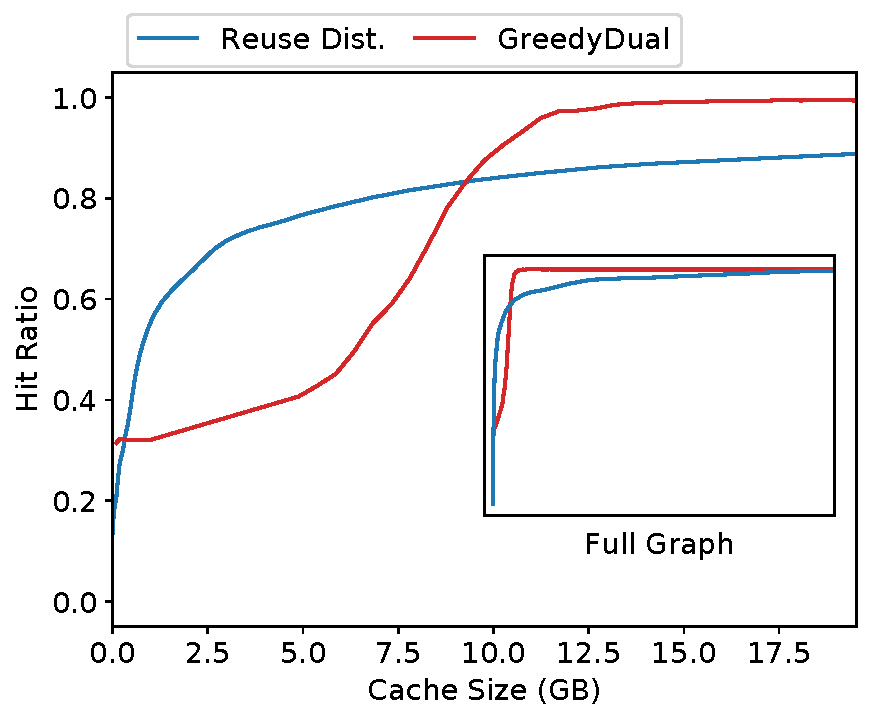
\includegraphics[width=0.5\textwidth]{faascache/faas-keepalive-20/graphs/rep-funcs-392/hit-ratio-392-b.pdf}
  \caption{Hit ratio curve using reuse distances show slight deviations from the observed hit ratios due to dropped requests at lower sizes, and concurrent executions at higher sizes.}
  \label{fig:hrc}
\end{figure}

\paragraph{Limitations of the Caching Analogy.}
The error in hit-ratios with the reuse-distance approach in Figure~\ref{fig:hrc} highlights an important facet where caching does not fully map to FaaS.
The main difference is due to the limitations on the concurrent execution of functions: 
caching deals with unique objects, whereas there can be  multiple containers for a function. 
%
At lower cache sizes, a high miss rate results in higher server load, and hence a higher number of dropped requests, that the classical reuse-distance approaches do not capture.
If all warmed containers of a function are in use, then a new invocation results in a cold-start---which would be counted as a cache ``hit''.
Thus at lower sizes, the real hit-ratio is lower than the ideal. 
At larger sizes, \emph{multiple} containers corresponding to concurrent invocations of a function will be present, which results in a deviation from the hit-rate curve. 
%: which is again different from the caching model where objects are unique. 
Reconciling these differences is an interesting area of future work. %but does not impact our work significantly. 
However, we note that hit-ratio curves are only used for coarse-grained allocation, and small deviations result in slight under or over provisioning. 
Moreover, our dynamic allocation policy described next can reduce these errors using proportional control. 

%\prat{Difference in two curves: could be because of multiple containers for a function, which is different from caching. So for larger cache sizes, the hit-ratio is higher. For lower sizes: it is lower because of dropped requests and not being able to handle the concurrent accesses which is not true with caching. So this is some sort of a negative result, or an area for future work.}


\subsection{Elastic Dynamic Scaling}
\label{subsec:dynamic}

We also use the hit-ratio curve approach for a \emph{dynamic} auto-scaling policy that adjusts the server size based on workload requirements. 
%
We assume that the FaaS server backend is running functions as containers either inside a virtual machine (VM), or is sharing the physical server with other cloud applications. 
In either case, it is important to be able to reclaim unused keep-alive cache resources and reduce its footprint, in order to increase the efficiency of the cloud platform. 

Our vertical elastic scaling policy is simple and is intended to demonstrate the efficacy of a general caching based approach. 
We implement a  proportional controller~\cite{pid-wiki} which periodically adjusts the VM memory size based on the rate of cold-starts.  
Thus during periods of low rate of function invocations (i.e., arrival rate), the cache size can be reduced. 
This may \emph{increase} the miss-ratio---but we care about the cold-starts (i.e., misses) per second, which is product of miss-ratio and invocations per second.
Our controller monitors the arrival and cold-start rate, and uses the hit-ratio curve to decrease or increase VM size dynamically. 
We use VM resource deflation~\cite{deflation-eurosys19} to shrink or expand the VM by using a combination of hypervisor level page swapping, or guest-OS memory hot-plug and unplug. 


Assume that we have a target miss speed (number of cold-starts/misses per second).
For instance, this target value can be a product of the desired hit-ratio, $h$, and the average function arrival rate for the entire workload trace, $\bar{\lambda}$. 
Periodically, we monitor the exponentially smoothed arrival rate $\lambda$, and the observed miss speed.
Our proportional controller adjusts the cache size in order to reduce the difference between the actual vs. target miss speed.
This error is used to compute the new \emph{miss rate}, $m$, and the associated cache size $c'$ as follows:
\begin{align}
  \label{eq:dyn}
%  m & = \frac{\bar{\lambda}}{\lambda}*h \\
  \text{HR}(c') & = 1-m = 1 - h\frac{\bar{\lambda}}{\lambda}
\end{align}

\noindent The new cache size $c'$ is then determined by inverting the hit-rate function $\text{HR}$.
Our vertical scaling controller is designed for coarse-grained VM size adjustments, and only tracks the workload at time granularities of several minutes. 
Our intent with this policy is to not be overly aggressive with the capacity changes, but only to capture the coarse diurnal effects. 
Therefore, we use a large error deadband: the cache size is only updated if the error is more than 30\%. 
%More sophisticated, predictive and reactive auto-scaling policies from web-clusters~\cite{gandhi2012autoscale} can be also be adapted. 
Finally, the memory scaling can also be combined with cpu auto-scaling based on the function arrival rate, using classical predictive and reactive auto-scaling techniques found in web-clusters~\cite{gandhi2012autoscale}. 

\paragraph{Online adjustments.} %rev1
Our policies rely on the \emph{aggregate} function characteristics, which is used for constructing the hit-ratio curve. 
Once done, the traffic intensity (invocations per second) can change.
We primarily assume that the probability distribution of function characteristics such as their frequency and size, does not significantly change.
However, our dynamic scaling policy can adjust to changes in the traffic intensity (invocations per second). 
In other words, we assume that the future traffic is going to be similar to the past, which is the basis of the timeseries-forecasting based policies (such as in ~\cite{shahrad_serverless_2020}), and is the fundamental principle underlying caching in general. 
%
Our provisioning policies are not completely online, since they have a preparation phase for constructing the hit-rate curves. 
A ``drift'' in function characteristics is fixed by periodically updating the hit-ratio curve, which we currently do once per week. 
Online hit-ratio curves can also be constructed, and adapting techniques such as ~\cite{zhang2020osca} is part of our future work.





% Let the exponentially smoothed arrival rate of functions be $\lambda$. 

% The hit-ratio curve constructed for the static provisioning is applicable for the overall workload for the average arrival rate $\bar{\lambda}$.
% For the elastic scaling, we monitor the exponentially smoothed arrival rate, $EWMA(\lambda)$, and scale up or down if it is more than one standard deviation from $\bar{\lambda}$. 
% If $\lambda < \bar{\lambda}$, we scale the server's memory down by $\delta(m)$, which is determined based on the cache hit ratio curve to meet the average or the set number of misses per second. 


% Let current cache size be c, and load be $\lambda$.
% In general, the misses per second is given by $m = (1-HR(c))\lambda$.
% The goal is to keep this constant, that is $m = \bar{m}$.
% If the new cache size is $c'$, then we have: $(1-HR(c'))\lambda  = (1-HR(c))\bar{\lambda}$
% \begin{equation}
%   \label{eq:dyn} 
%   HR(c') = 1- \dfrac{(1-HR(c))\bar{\lambda}}{\lambda} 
% \end{equation}
% We use the hit-rate curve to thus find $c'$ that yields the hit-rate on the right hand side of the above equation.  

% tgt-miss-rate = avg-lambda/lambda*miss-ratio 


%%% Local Variables:
%%% mode: latex
%%% TeX-master: "paper"
%%% End:


\section{Implementation}

We have implemented the keep-alive and the provisioning policies as part of our FaasCache framework built on top of OpenWhisk (Figure~\ref{fig:sys}). 

\begin{figure}[t]
  \centering
  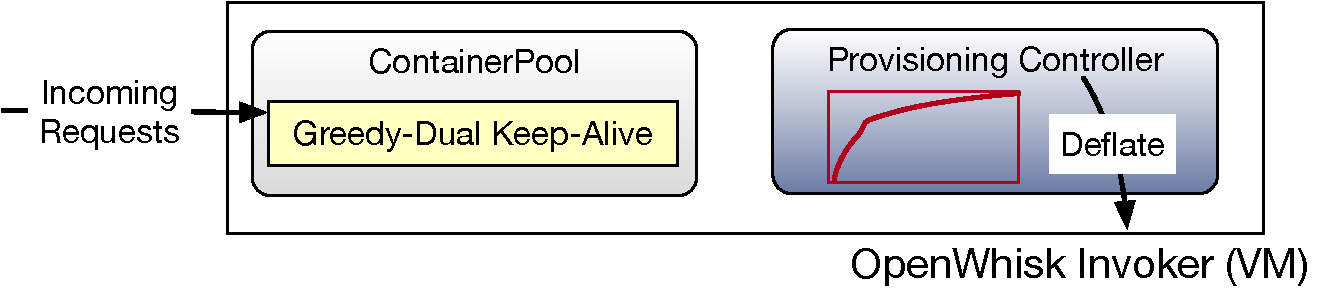
\includegraphics[width=0.95\textwidth]{faascache/faas-keepalive-20/figures/faascache.pdf}
  \caption{FaasCache system components. We build on OpenWhisk and augment it with new keep-alive policies and a provisioning controller. }
  \label{fig:sys}
\end{figure}

\noindent \textbf{Keep-Alive.}
FaasCache replaces the default OpenWhisk TTL-based keep-alive policy with the Greedy-Dual-Size-Frequency approach. 
For each initialized container, we assign and maintain the keep-alive prioritized ContainerPool, which is only a 100-line Scala modification. 
%Initialized containers are managed by the ContainerPool.
%\emph{Interesting aspects of priority calculation?} How is size, clock, frequency, cost, etc. computed? How does the impl differ from the idealized description? 
Each invocation of a function (OpenWhisk action) in ContainerPool records the launch time and when results are returned.


If the container was prewarmed before the invocation arrived, we record it as the function's warm runtime.
For new functions, the initialization overhead is captured and assumed to be the worst-case runtime until a warmed invocation is recorded. % is approximated as the minimum overhead of Docker and OpenWhisk's Python runtime initialization.
In the subsequent invocations, the initialization overhead is computed by subtracting the cold from the warm time. 
%Otherwise it was a cold start.
%The maximum cold and warm runtimes are kept per function to compute the priority.
%Size is simply the number of megabytes of memory OpenWhisk preallocates to the action's container, and
The function's frequency and clock value are updated with each request.
If the last container of a function is evicted, its cold and warm runtimes are stored and used to compute priority for its future invocations. 
%
To preserve the invocation fast-path, the ContainerPool is not kept sorted by priority. 
%Priorities are computed when an eviction needs to be made to reclaim memory.
Instead, it is sorted by priorities only during evictions, when the lowest priority container(s) are terminated.
%
We batch eviction operations to optimize the slow-path: we evict multiple containers to reach a certain free resource threshold (1000 MB is the current default). 

%rev 1
In the future, we intend to implement a similar design that is found in the Linux kernel page eviction. A separate thread (analogous to kswapd) can be used to periodically sort the containerpool list and asynchronously evict containers, so that eviction is not on the critical path. 

%All of an action's containers share one priority, regardless of the last time each ran an invocation.

% \prat{How are the values inferred?}
% New functions always replace old functions in the ContainerPool, so the priority of newly inserted containers doesn't matter. 
% After the second invocation of a function, its initialization overhead is inferred as the difference between the cold (first) and warm (subsequent) invocations. 
% Memory usage of the container is gathered via {\em Docker stats?\/}.



\noindent \textbf{Provisioning.}
For the static provisioning, we compute the reuse distance distribution for a given workload trace, and assume stationarity --- that it will be applicable on similar future workloads. 
We compute the reuse distances conventionally, by examining all reuse-sequences.
The dynamic provisioning controller runs periodically (every 10 minutes), to deflate or inflate the VM size, if the cold start rate deviates from the target significantly (by more than 30\%).
When the VM has to be shrunk, we use cascade deflation~\cite{deflation-eurosys19}.
We shrink the ContainerPool first, and reclaim the free memory using guest OS-level memory hot-unplug and hypervisor-level page swapping. 
%This approach is based on cascade deflation proposed in~\cite{deflation-eurosys19}. 

%Optimizations such as SHARDS that can significantly reduce the running time by sampling a small fraction of the functions, were found to be inadequate due to the wide disparity in the function sizes.
%The efficacy of sampling based techniques like SHARDS has mainly been empirically established only for fixed-sized objects. 


\noindent \textbf{Keep-alive Simulator.}
We have implemented a trace-driven discrete event simulator for implementing and validating different keep-alive policies.
Our simulator is written in Python in about 2,000 lines of code, and implements the various variants described in Section~\ref{subsec:variants}. 
It allows us to determine the cache hit ratios and the cold start overheads for different workloads and memory sizes.
Additionally, it also implements the static and dynamic provisioning policies for adjusting server size.

%%% Local Variables:
%%% mode: latex
%%% TeX-master: "paper"
%%% End:


\section{Experimental Evaluation}

% section Evaluation
\label{sec:eval}


We now present the experimental evaluation of our caching-based keep-alive technique by using function workload traces and serverless benchmarks.
Our goal is to investigate the effectiveness of these techniques under different workload and system conditions. 


\begin{figure*}
  \centering
\subfloat[ Representative functions.     \label{fig:rep-trace-exec}]
{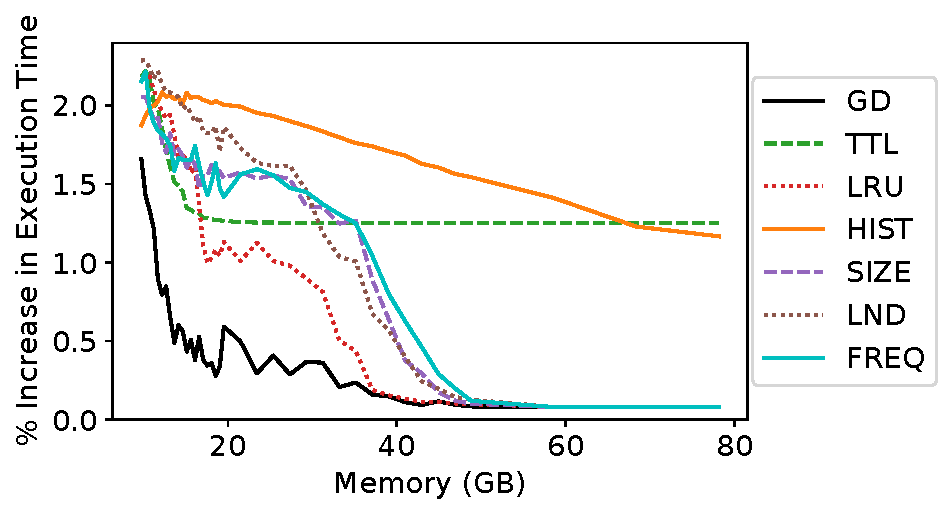
\includegraphics[width=0.37\textwidth]{faascache/faas-keepalive-20/graphs/rep-funcs-392/exec_inc_mem-392-legend.pdf}}
  \hfill 
    \subfloat[Rare functions.     \label{fig:rare-trace-exec}]
{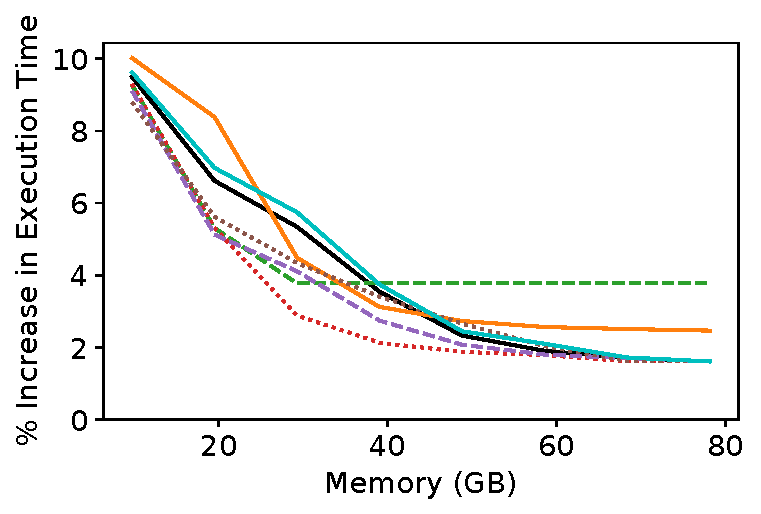
\includegraphics[width=0.3\textwidth]{faascache/faas-keepalive-20/graphs/rare-funcs-1000/exec_inc_mem-1000.pdf}}
\hfill 
  \subfloat[Random sampling.      \label{fig:random-trace-exec}] {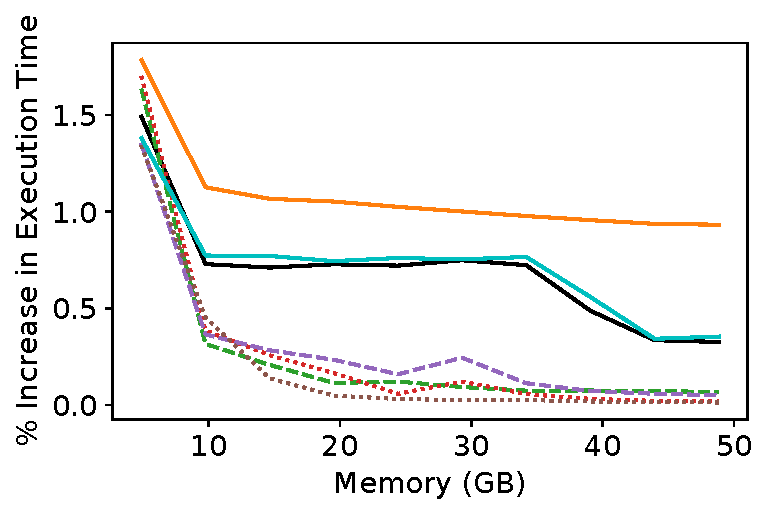
\includegraphics[width=0.3\textwidth]{faascache/faas-keepalive-20/graphs/random-funcs-200/exec_inc_mem-200.pdf}}
\caption{Increase in execution time due to cold starts for different workloads derived from the Azure function trace.}
\label{fig:exec-overheads-all}
\end{figure*}


\begin{figure*}[t]
  \centering
%  \vspace*{\myfigspace}
%  \begin{minipage}[c]{0.7\linewidth}
  \subfloat[Representative functions.\label{fig:rep-trace-cold}] {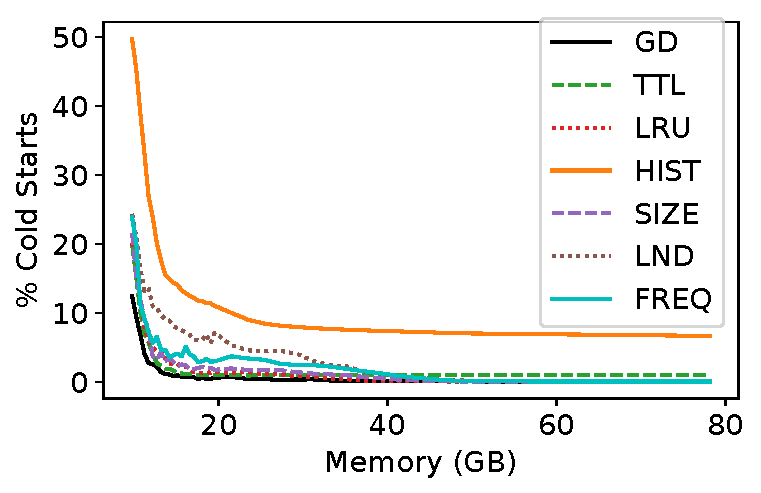
\includegraphics[width=0.33\textwidth]{faascache/faas-keepalive-20/graphs/rep-funcs-392/cold_drop_mem-392-legend.pdf}}
  \hfill
    \subfloat[Rare functions. \label{fig:rare-trace-cold}] {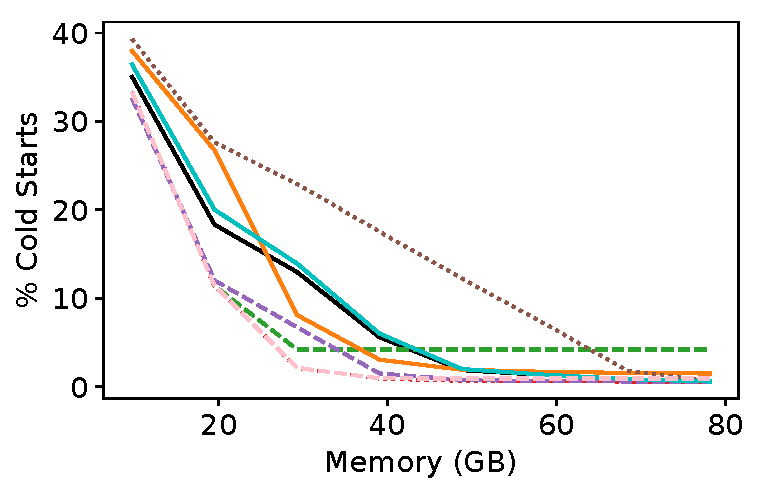
\includegraphics[width=0.33\textwidth]{faascache/faas-keepalive-20/graphs/rare-funcs-1000/cold_drop_mem-1000.pdf}}
  \hfill
  \subfloat[Random sampling. \label{fig:random-trace-cold}]
  {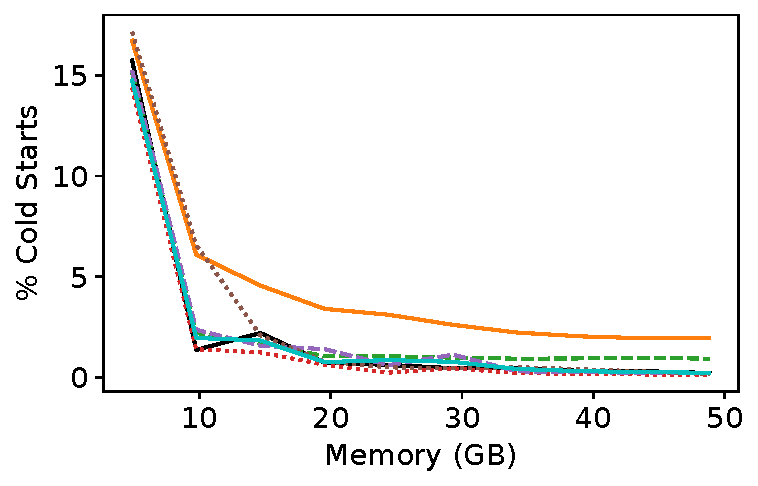
\includegraphics[width=0.33\textwidth]{faascache/faas-keepalive-20/graphs/random-funcs-200/cold_drop_mem-200.pdf}}
    \caption{Fraction of cold starts is lower with caching-based keep-alive. } % for different samples of the Azure function trace.}
      \label{fig:cold starts-all}
%    \end{minipage}
%    \hfill
%    \begin{minipage}[c]{0.29\linewidth}
 %      \begin{figure}
 %     \end{figure}
%    \end{minipage}
\end{figure*}


%%%%%%%%%%%%%%%%%%%%%%%%%%%%%%%%%%%%%%%%%%%%%%%%%%%%%%%%%%%%
\noindent \textbf{Setup, Workloads, and Metrics.}
%
For evaluating different keep-alive performance with different workload types, we use different trace samples from the Azure Function trace~\cite{shahrad_serverless_2020}, which contains execution times, memory sizes, and invocation-timestamps for more than 50,000 unique functions. 
Since our goal is to examine performance at a \emph{server} level, we use smaller samples of this trace for realistic server sizes, and replay them in our discrete-event keep-alive simulator. 
This also allows us to examine the behavior with different \emph{types} of workloads, which is important because our keep-alive policies are designed to be general and workload-agnostic.
We use the following three trace samples (more details in the Table~\ref{tab:trace-deets}): \\
\noindent \textbf{RARE:} A random sample of 1000 of the rarest, most infrequently invoked functions. These functions will usually result in cold starts under a classic 10 minute TTL.  \\
% mention 75% percentile detail?
\noindent \textbf{REPRESENTATIVE:} A sample of 400 functions, sampled from each quartile of the dataset based on frequency---yielding a more representative sample with higher function diversity. \\
\noindent \textbf{RANDOM:} A random sample of 200 functions.

% The FaasCache system is evaluated in Section~\ref{subsec:ow-eval}.
Functions from the FunctionBench~\cite{kim_functionbench_2019} suite are used for generating a realistic workload. 
A single server with 250 GB RAM and 48-core Intel Xeon Platinum 2.10 GHz CPUs is used for running all functions. The server is running modified OpenWhisk (i.e., FaasCache), and Ubuntu 16.04.5. 

\begin{table}
  \centering
  \caption{Size and inter-arrival time (IAT) details for the Azure Function workloads used in our evaluation.}
  \begin{tabular}{lrrr}
    \hline 
    Trace & Num Invocations & Reqs per sec & Avg. IAT \\
    \hline
    Representative & 1,348,162 & 190 /s & 5.4 ms \\
    Rare & 202,121 & 30 /s & 36 ms \\
    Random & 4,291,250 & 600 /s & 1.8 ms \\
    \hline
  \end{tabular}
  \label{tab:trace-deets}
\end{table}



\paragraph{Adapting the Azure Functions Trace.}
The format of the original Azure Function trace~\cite{shahrad_serverless_2020} requires some additional pre-processing and extrapolation for generating a workload.  
The full dataset consists of 14 days of function invocations, and billions of individual invocations. We use the first day's data, and do not consider functions that are never reused (i.e., with less than two invocations). 

The original trace provides memory consumption at the \textit{application} level---with the application made up of multiple functions.
Therefore, we evenly split the memory allocation between all functions in an application.
The dataset provides invocations in minute-wide buckets.
When injecting/replaying the workload, if there is only one invocation in a minute-bucket, it is injected at the beginning of the minute. 
For multiple invocations, they are equally spaced throughout the minute. 

%
The cold start overhead of each function is estimated as {\texttt maximum - average} runtime, and the execution times provided in the dataset are used for this computation. 
The dataset does not account for certain important sources of cold start overheads such as execution environment creation (e.g., Docker).
This unfortunately underestimates the cold start overheads.
However, because it applies uniformly to all functions, it preserves the relative performance of the different keep-alive policies, and does not affect the cache hit ratios. 
%

%These cold start overheads are generally constant, 

%This may not capture all the sources of cold start overhead such as the execution environment creation (e.g., Docker) and 

We are interested in two metrics: the cold start ratio; and the average increase in the execution time due to cold starts.
The increase in execution time is computed by averaging across all function invocations. 

%The latter captures the heterogeneity in function initialization overheads and invocation frequencies. 
%For estimating the time each function spends in explicit initialization, using the workload trace we subtract each functions' average runtime from its maximum runtime. 
%The dataset timings do not include provider overhead, so this initialization time is entirely due to application code.

%%
%Provider cold start overheads can be up to several seconds long, and take up the plurality of a function's execution time.
%Because the dataset does not include provider overhead, it is impossible to assign a realistic number to this cost.
%With these large penalties are not in our simulations, we therefore assume it as 0, but in reality the overhead is roughly constant.
%This causes the global increase in execution time to be smaller than it would be otherwise.
%Including a non-zero cold start cost would apply uniformly across all functions, and thus not change eviction priorities relative to one another.
%The cache hit ratio in Figure~\ref{fig:cold starts-all} would remain unchanged, and the Y-axis (the global increase in execution time) of Figure~\ref{fig:exec-overheads-all} would be scaled up relative to the chosen cold start overhead.
%%

% Using variable, real-world, times would require knowing or randomly assigning the runtime of functions, and would still require stochasticity as provider latency is not constant. 

% Not explaining this in the paper was our biggest “oops”: and there’s a few sources of confusion.
% Here is what we assumed: the dataset doesnt include container startup time, but the included function execution time captures both the function-initialization time (importing packages etc.), and the actual execution.
% So the assumption is that the Max execution time was due to this initialization overhead (which we include in the cold start overhead in our paper).
% The “time functions take to execute after they are ready to run” added to our confusion: we assumed this meant that it is the time when the control is transferred to the FaaS runtime inside the container: which would still incorporate all actual function initialization overheads.
% A contributing factor to making this assumptions was that most OpenWhisk applications do not have a strict explicit initialization, so it is in general not possible to know when a function is truly ready to execute non-idempotent code. 

% And so we end up with pretty small startup overheads, which can be seen from our Figure 5.
% Including container startup time and other overheads would make little difference to relative performance, since the extra overhead would apply to all functions.
% For instance, adding a constant startup penalty for all functions doesnt change their eviction priorities.
% The cache hit ratio (our Figure~\ref{fig:cold starts-all}) would remain unchanged, and the Y-axis of Figure~\ref{fig:exec-overheads-all} would be scaled up depending on the chosen cold start overheads. 

\begin{comment}
Our simulator evaluation uses real-world FaaS usage data from the recently released Azure Function trace~\cite{shahrad_serverless_2020}. 
The entire trace consists of tens of thousands of functions with billions of invocations, making it intractable to simulate the entire dataset.
Trace sampling methodology is important to capture the characteristics of the overall trace, and the scenarios where FaasCache is most effective.
Over half of all functions have an interval arrival time (IAT) over 30 minutes, where IAT is defined as execution time + idle time, guaranteeing them to always have cold starts when using a simple TTL eviction policy.
A tiny 1\% of functions account for nearly 90\% of all invocations, with an IAT of under a minute. 
% Therefore, smaller samples 
Given these extreme disparities, smaller samples must match behaviors of the larger dataset to show their effectiveness.
The full Azure trace can be suitably handled by a cluster of servers, in which case the system behavior is influenced by load-balancing and sharding policies, which our work is orthogonal to.
%Explain the rationale here. 
We generate three day-long traces using the Azure Functions dataset to showcase the effectiveness of FaasCache.
\prat{Insert reuse distance vs. time heatmaps for all these traces in the appendix along with table describing: number of fns, total invocations, avg. inter arrival time, etc.}
\end{comment}

%%%%%%%%%%%%%%%%%%%%%%%%%%%%%%%%%%%%%%%%%%%%%%%%%%%%%%%%%%%%
\subsection{Trace-Driven Keep-Alive Evaluation}

In this subsection, we use the Azure function traces to evaluate different keep-alive policies in our discrete-event simulator. 
% Primary Comparison? Competitors? 
We compare all caching-based variants against the default keep-alive policy in OpenWhisk (10 minute TTL).
% rev 1
When the server is full, this TTL policy evicts containers in an LRU order.
We also evaluate different Greedy-Dual variants: GD is our GDSF policy described in Section~\ref{subsec:gdsf}.
The others are the caching-based variants described in Section~\ref{subsec:variants}: LND is Landlord, and FREQ is LFU. 


%rev 1 
We also compare against the histogram-based keep-alive policy in~\cite{shahrad_serverless_2020}, which is the state of the art technique.
% Section 4.2 of serverless paper 
We have reproduced this policy (HIST) from the details in the paper, and have implemented it in a ``best-effort'' manner without any knowledge of the optimizations in the actual implementation.
This is effectively a ``TTL+Prefetching'' policy: it uses a histogram of \emph{inter-arrival times} to predict future function invocations and eagerly evict warm functions.
It uses timeseries forecasting to capture temporal locality, but does not consider the other function characteristics such as function size and initialization cost. 
The IAT, computed by taking a function's execution time plus the subsequent idle time, between each actual invocation is recorded in minute granularity buckets, tracking up to four hours between executions.
The policy uses ARIMA modeling for those invocations that fall outside this four hour window, we chose not to implement this specific feature due to its complexity, and the fact that it accounted for a minor fraction (\textasciitilde 0.56\%) of all invocations.
From these buckets, a function's coefficient of variation (CoV) is calculated using Welford's online algorithm~\cite{welford}. 
When the function's IAT is predictable (CoV $\leq 2$), the function's historical/customized preload and TTL time are used.
Otherwise, the function has a generic TTL of two hours. 
When an invocation is anticipated, it is brought into memory and kept there until its TTL expires.
A function is evicted when the policy predicts it will not have an invocation in the near future. 
%We chose not to implement the ARIMA modeling for IAT's exceeding four hours for simplicity and the fact it is only applicable to a tiny number of functions.
% \textbf{More details. Histogram size? When created? Online? }


%
The increase in execution time for different traces and for different cache sizes is shown in Figure~\ref{fig:exec-overheads-all}.
% How is this measured?
The increase in execution time is the cold start overheads averaged across all invocations of every function, and captures the user-visible response-time. 
%

For the representative trace (Figure~\ref{fig:rep-trace-exec}), Greedy-Dual reduces the cold start overhead by more than $3\times$ compared to TTL for a wide range of cache sizes (15--80 GB). 
Interestingly, it is able to achieve a low overhead of only 0.5\% at a much smaller cache size of 15GB, compared to other variants, which need 50 GB to achieve similar results---a reduction of cache size by more than $3\times$. 
%
For rare functions (Figure~\ref{fig:rare-trace-exec}), caching-based approaches such as LRU  reduce the cold start overhead by $2\times$ compared to TTL for cache sizes of 40--50 GB. 
This shows that for rare functions, recency is a more pertinent characteristic, and the complex four-way tradeoff used in Greedy-Dual is not necessarily ideal in all workload scenarios. 
For this workload, the HIST policy outperforms TTL, as reported in~\cite{shahrad_serverless_2020}. 
However, it results in 50\% higher cold start overhead compared to caching-based approaches.
Furthermore, because HIST uses only inter-arrival times, it is unable to perform well with heterogeneous representative workloads  (Figure~\ref{fig:rep-trace-exec}). 


Finally, the randomly sampled trace has a large number of infrequent functions because of the low probability of selecting the heavy-hitting functions.
In Figure~\ref{fig:random-trace-exec}, the recency component again dominates, and we see LRU outperforming other variants. 
The equivalence of LRU and TTL-based caching for rare objects has been noted~\cite{basu2017adaptive,jiang2018convergence}, which explains their similar behavior seen in Figure~\ref{fig:random-trace-exec}. 
%closeness of TTL and LRU performance for rare functions in our result. 


\noindent \emph{\textbf{Result:} For representative, diverse workloads, our GD policy can improve the performance and shrink cache sizes by up to $3\times$. For more homogeneous workloads, LRU can outperform current TTL-based approaches by $2\times$.}

%%%
% rev 1 
We can observe from Figure~\ref{fig:exec-overheads-all} that the increase in execution time is generally small ($<10\%$).
This is because of two main factors: the evaluation metric chosen, and the properties of the workload trace. 
The execution time is averaged across \emph{all} function invocations.
However, serverless workloads consist of a large number of very frequently invoked functions. 
The performance of these functions is generally not affected by keep-alive policies, since any policy is going to keep them in the cache because of their high frequency. 
Thus, the difference between non-work-conserving policies such as TTL and Greedy-Dual is masked because of the frequent and popular functions. 
For instance, the average inter-arrival time for all three workloads is less than 36ms, or about 27 function invocations per second. 
Thus, the server is overloaded, and TTL does well even though it is not work-conserving. 
As the IAT grows, the effectiveness of work-conserving caching-based approaches increases compared to TTL, as we shall see in the next subsection. 

%%%%
%While Figure~\ref{fig:exec-overheads-all} focuses on the average increase in execution latency, keep-alive can also reduce the tail latency of functions. Cold start 

%%%%

We see a similar relation and behavior in the miss-ratio curves shown in Figure~\ref{fig:cold starts-all}. 
Due to function heterogeneity, the cold start overheads are not strictly correlated with cache miss ratios, and thus the differences between policies is different compared to the previously described actual cold start overheads. 
% \prat{Write after colors are fixed.}
Classic miss-ratio curves do not consider the miss \emph{cost} (i.e., initialization cost), which is an important metric that is optimized by the Greedy-Dual approach.
Thus, in general, even in object caching contexts, miss-ratio curves deviate from the actual performance---a behavior that we also observe. 

%%%%%%%%%%%%%%%%%%%%%%%%%%%%%%%%%%%%%%%%%%%%%%%%%%%%%%%%%%%%
\subsection{OpenWhisk Evaluation}
\label{subsec:ow-eval}



\begin{figure}
  \centering
  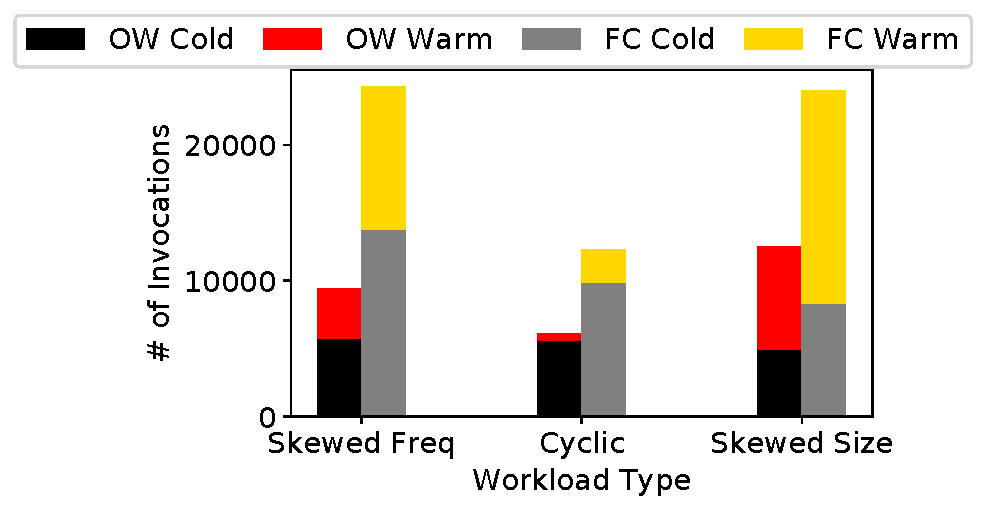
\includegraphics[width=0.6\textwidth]{faascache/faas-keepalive-20/graphs/litmus_tests/litmus_2_stacked.pdf}
  \caption{FaasCache runs 50 to 100\% more cold and warm functions, for skewed workload traces.}
  \label{fig:litmus_2}  
\end{figure}


In this subsection, we evaluate the performance of the FaasCache system on real functions. 
We focus on the performance of FaasCache's Greedy-Dual keep-alive implementation, and compare it to the vanilla OpenWhisk system which uses a 10 minute TTL.


% rev1 1
In contrast to the previous subsection in which we showed the average performance for different cache sizes, we will now also focus on the inverse problem: for a fixed server size, how much more load can be handled with FaasCache? 
By leveraging Greedy-Dual caching, FaasCache is able to reduce cold starts. 
This also reduces the number of \emph{dropped} requests. %

OpenWhisk buffers and eventually drops requests if it cannot fulfill them.
Because FaasCache more effectively selects evictions, its higher hit rate results in functions finishing faster, allowing more functions to be executed in the same time frame.  
%
\begin{table}
  \centering
  \caption{FaaS workloads are highly diverse in their resource requirements and running times. The initialization time can be significant and is the cause of the cold start overheads, and depends on the size of code and data dependencies.}
  \begin{tabular}{lrrr}
    \hline 
    Application & Mem size & Run time & Init. time \\
    \hline
    ML Inference (CNN) & 512 MB & 6.5 s & 4.5 s \\
    Video Encoding & 500 MB & 56 s & 3 s \\
    Matrix Multiply & 256 MB & 2.5 s & 2.2 s \\
    Disk-bench (\texttt{dd})  & 256 MB & 2.2 s & 1.8 s \\
    Image Manip & 300 MB & 9 s & 6 s \\
    Web-serving & 64 MB & 2.4 s & 2 s \\
    Floating Point & 128 MB & 2 s & 1.7 s \\
    \hline
  \end{tabular}
  % \vspace*{\myfigspace}
  \label{tab:fc:workloads}
  %\vspace*{\myfigspace}
\end{table}

To examine the effect of Greedy-Dual keep-alive on cold start and dropped requests, we use a workload trace comprising of four different functions: Disk-bench, ML inference, Web-serving, and Floating-point, described in Table~\ref{tab:fc:workloads}.

In Figure~\ref{fig:litmus_2}, we use different kinds of \emph{skewed} workloads: with a single function having a different frequency, a cyclic access pattern, and a skewed workload with 2 sizes. 
We see that FaasCache's keep-alive can increase the number of warm invocations by between 50 to 100\% compared to OpenWhisk's TTL.
The difference in the total number of requests served (warm+cold) is because OpenWhisk drops a significant number of requests due to its high cold start overhead and resultant system load. 
%
Thus with FaasCache, the total number of requests that are served also increases by $2\times$. 

%rev 1 above 
%Interestingly, OpenWhisk drops a significant number of requests, which is the cause of the different total served requests. 
%

% The impact on the different function performances can be seen in Figure~\ref{fig:faasbench}.
% For this figure, to generate the workload, the first three functions have an inter-arrival time of 1500 ms, and the fourth (floating-point) has a lower IAT of 400 ms. 

%a disk-based one, web-page serving, floating-point trigonomotry operations in numpy, and a convolutional neural network inference (TensorFlow with which model?). % A detailed description of these workloads is required.

% Explain what is the iat distribution and (other details? ).


% 32 GB wted_increase vanilla 11.964% cache 11.528%
% 48 GB wted_increase vanilla 6.184% cache 0.624%


\begin{figure}[t]
  \centering
\includegraphics[width=0.6\textwidth]{faascache/faas-keepalive-20/graphs/litmus_tests/faasbench_48_cold_hot-legend.pdf}
\caption{FaasCache increases warm-starts by more than $2\times$, which also reduces system load and dropped functions.}
\label{fig:faasbench}
\end{figure}


\begin{comment}
\begin{figure}[t]
  \centering
\subfloat[48 GB   \label{fig:faasbench-stacked-48}]
{ \includegraphics[width=0.3\textwidth]{../graphs/litmus_tests/faasbench_48_cold_hot-legend.pdf}}
\hfill 
  \subfloat[32 GB   \label{fig:faasbench-stacked-32}]
{  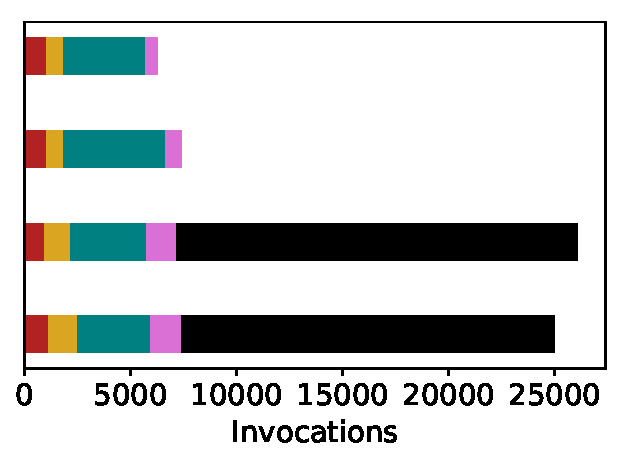
\includegraphics[width=0.17\textwidth]{../graphs/litmus_tests/faasbench_32_cold_hot.pdf}}
\caption{Impact of keep-alive on different function types.}
\label{fig:faasbench}
\end{figure}
\end{comment}

% Figure~\ref{fig:faasbench-stacked-32} shows the number of cold and dropped requests for the different functions, with a medium cache size of 32 GB.
% This setup is intended to evaluate our system in resource constrained environments.
% We see that dropped requests dominate, and FaasCache's more effective keep-alive serves 45\% of requests, while OpenWhisk only serving ~40\%.
% At the same time, warm starts improve 17\% using FaasCache.


Next, we use the skewed frequency workload and use functions from Table~\ref{tab:fc:workloads} to evaluate the impact on real applications. 
%The impact on the different function performances can be seen in Figure~\ref{fig:faasbench}.
To generate the workload, the CNN, DD, and Web-serving functions have an inter-arrival time of 1500 ms, and the Floating-point function has a lower IAT of 400 ms. 
%
Figure~\ref{fig:faasbench} shows the breakdown of different function invocations for this workload on a 48 GB server.
Interestingly, OpenWhisk drops a significant number (50\%) of requests due to the its high cold start overheads.
FaasCache increases the warm requests by more than $2\times$. 
Interestingly, the \emph{distribution} of warm starts is also different. 
FaasCache's Greedy-Dual policy prioritizes functions with higher initialization times, but penalizes those with large memory footprints. 
Because the floating-point function has a high initialization overhead (Table~\ref{tab:fc:workloads}), it sees a $3\times$ increase in hit-ratio compared to OpenWhisk.
\emph{In practical terms, the improvement in keep-alive results in a $6\times$ reduction in the application latency.
}
%The ML inference function has an 8\% lower warm hit rate than the other functions, as it gets de-prioritized because of it's high memory needs.


%When the cache size is increased to 48 GB (Figure~\ref{fig:faasbench-stacked-48}), FaasCache doesn't drop a single request, while OpenWhisk still can't serve 50\% of them.
%For the same workload, Figure~\ref{fig:faasbench-stacked-32} shows the distribution of cold and warm starts for a larger cache size of 32 GB.
%The number of warm starts increases by nearly 20\% compared to OpenWhisk.
% FaasCache's Greedy-Dual policy prioritizes functions with higher initialization times, the CNN function sees a 53\% higher warm starts, wheres Z function only sees X\% increase compared to OpenWhisk. 
% The floating point function has a very high initialization overhead (1.7 of the total 2 seconds), and thus sees its warm-start rate increase the most, by 40\%. 

\begin{comment}
At a smaller cache size of 32 GB shown in Figure~\ref{fig:faasbench-stacked-32}, the number of dropped requests dominate.
This setup is intended to evaluate our system in resource constrained environments.
FaasCache's more effective keep-alive serves 45\% of requests, while OpenWhisk drops nearly 60\%.
Warm-starts increase by 17\% with FaasCache. 
\end{comment}

\noindent \emph{\textbf{Result:} FaasCache can increase the number of warm-starts by $2\times$ to $3\times$ depending on the function initialization overheads and workload skew. This results in lower system load, which increases the number of requests FaasCache can serve by $2\times$.}

%\prat{CPU Graph not required, but just the average numbers will do.}

%%%%%%%%%%%%%%%%%%%%%%%%%%%%%%%%%%%%%%%%%%%%%%%%%%%%%%%%%%%%
\subsection{Effectiveness of Provisioning Policies}
All our previous results have been with a statically allocated server, and 
we now illustrate the effectiveness of our dynamic vertical scaling policy described in Section~\ref{subsec:dynamic}.
The goal is to dynamically adjust the cache size based on the workload. 
Our  policy seeks to keep the miss speed (cold starts per second) close to a pre-specified target. 
This is shown in Figure~\ref{fig:dynamic}---the target is 0.0015 misses per second. 
In this experiment, the cache resizing is done only when the miss speed error exceeds 30\%, and we can see that the cache size increases with the miss speed, and decreases with it. 
Without the dynamic scaling, a conservative provisioning policy would result in a constant, 10,000 MB size. 
In contrast, the average cache size with our proportional controller is less than 7,000 MB.
This 30\% reduction means that FaaS providers can reduce their provisioned resources without compromising on performance.
The freed-up resources can be used to accommodate additional cloud workloads (such as co-located VMs and containers). 
Our dynamic scaling is extremely conservative: increasing its agressiveness by reducing the error tolerance below 30\% will reduce  average server size,
%but cause a larger number of small memory-size  changes, which we wish to avoid.
but we seek to avoid the resultant small changes to memory-size to minimize fragmentation. 
%avoid why?? 

\begin{figure}[t]
  \centering 
  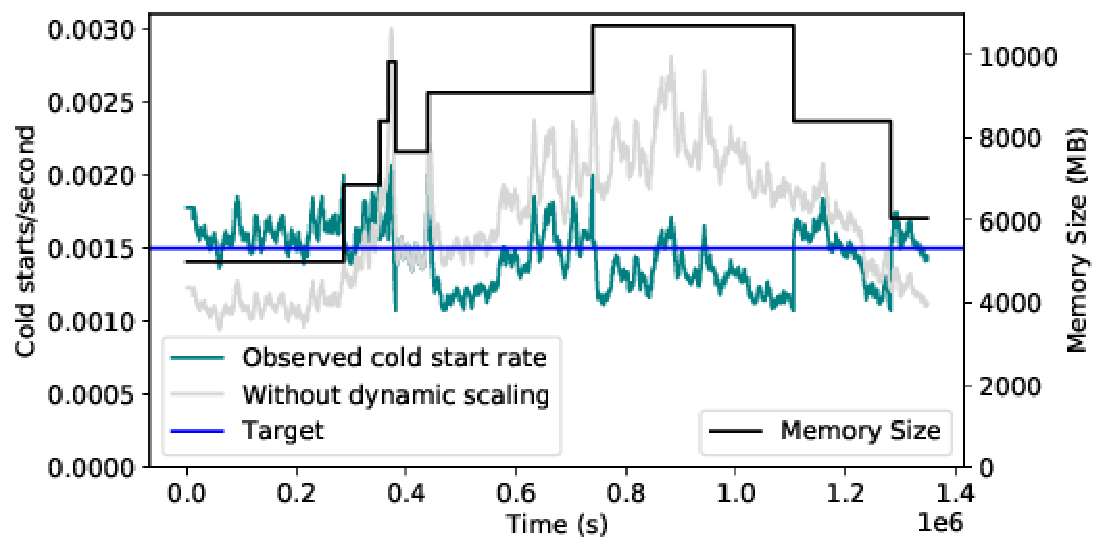
\includegraphics[width=0.6\textwidth]{faascache/faas-keepalive-20/graphs/dyn-scale-392-b.pdf}
  \caption{With dynamic cache size adjustment, the cold starts per second are kept close to the target (horizontal line), which reduces the average server size by 30\%. }
  \label{fig:dynamic}
\end{figure}

%%% Local Variables:
%%% mode: latex
%%% TeX-master: "paper"
%%% End:


\section{Related Works}
\label{sec:faascache-related}

% \section{Related Work}

% \noindent \textbf{Function Keep-alive.}
Mitigating cold starts is one of the central performance problems in FaaS, and has received commensurate attention in both academia and industry.
%
The initialization or startup time of functions can be reduced  by reducing container startup overheads~\cite{oakes_sock_2018,mohan_agile_2019, akkus_sand_2018}, or deploying functions inside ultra-light containers, VMs, or unikernels~\cite{unikernels,firecracker-nsdi20}.
%
While these mechanisms can reduce the cold start overhead associated with the virtual environment creation, other sources of overheads remain, such as losing all application initialized variables, cached files, etc.
As we have shown, keep-alive essentially serves the role of caching, and fast startup only reduces the ``miss'' penalty, and does not eliminate it.

% Rev 1 
Catalyzer~\cite{du2020catalyzer} implements new mechanisms for checkpointing and restoring application and sandbox state, which significantly reduce the initialization cost of functions deployed in their gvisor-based sandbox environment. 
Our approach is complementary to these techniques since we focus on retaining the entire execution environment instead of optimizations for restoring/recreating it. 
Keep-alive policies can be combined with these optimized mechanisms to improve system-wide performance even further. 

%for functions by forking a lightweight execution environment after function initialization. %still uses memory though?
%This reduces duplicate computation, 
%It uses a complementary set of techniques, since we tradeoff extra memory for simpler system and deployment complexity. 

Principled keep-alive policies for functions have recently gained attention: the recent dataset and policy from the Azure function trace~\cite{shahrad_serverless_2020} shows the importance and effectiveness of keep-alive policies. 
In contrast to our work, their policy does not take the function size into consideration and uses a time-series prediction approach (effectively capturing recency and frequency), and combines it with a predictive ``prefetching'' approach. 
As we have shown, function memory footprints are a crucial characteristic, and the use of caching allows the use of advanced analytical and modeling approaches for serverless computing in general. 
% rev 1 
Earlier work has focused on simple ``warm container pools''~\cite{lin_mitigating_2019}, in which Kubernetes cluster runs a certain number of warm containers for functions. 
Our caching-based policies take this one step further and decide \emph{which} container to keep-alive, and for how long. 
Polling to keep cloud functions warm has also been a popular method~\cite{warm2,warm1}.



%
Our work considers functions individually---function scheduling with DAG based approaches~\cite{carver_search_2019} is effective for function-chains, and are orthogonal and complementary to our work. 
%
Hiding function latency using data caching (such as redis) for database applications is investigated in~\cite{ghosh_caching_2019}. 
The ENSURE~\cite{ensure_acsos20} system handles keep-alive and resource provisioning for CPU resources using queuing theory techniques.
Our focus is on memory-constrained keep-alive and provisioning, and CPU-focused approaches are complementary to our work. 

\subsection{Comparative Works}

FaasCache has inspired a number of new caching policies, and of everything in this thesis has become the most popular system to reference and compare against.
Listed here are those that directly compare against FaasCache.
Heterogeneous FaaS workers~\cite{roy2022icebreaker} and predictive prewarming of containers~\cite{saha2024fase} can improve performance.
Edge computing has strict resource requirements, and uses a mix of scheduling and cache management to minimize cold starts~\cite{zhang2023online,chen2024cross}.
Invocations can also be intelligently scheduled, batched, and re-ordered to avoid cold starts~\cite{wu2024faasbatch,cai2024incendio}.

\begin{comment}
\noindent \textbf{Caching.}
Our choice of Greedy-Dual-Size-Frequency was motivated by the ease with which its parameters mapped to function keep-alive, in particular the frequency vs. size tradeoff.
Cache eviction algorithms have a long history, although the focus has predominantly on uniform sized objects (such as disk blocks, RAM pages, cache lines, etc.).
Certain caching optimizations relying on spatial locality (such as look-ahead and ARC) are not directly applicable to keep-alive. 
The size-aware cache algorithms and models used for web-caches, proxies, and CDNs form the basis of our work. 
Cache provisioning using hit/miss ratio curves is a common approach, and these curves can also be constructed dynamically, which is part of our future work.
%
\end{comment}

\begin{comment}

The Azure function traces and keep-alive approach 

Prior work has investigated reducing container startup overheads, which can reduce the 

\noindent \textbf{Usecases}

~\cite{cartas_reality_2019} questions the need for edge computing for ML inference, because of the decreasing inference latency and costs, and network latency becomes the primary bottleneck.

Berkeley view~\cite{jonas2017occupy, jonas_cloud_2019}

Interactive applications---RunBox ~\cite{glikson_runbox_2019}.

Data analytics with ServerMix~\cite{garcia-lopez_servermix_2019}

ExCamera

PyWren

Serverless analytics with Flint wtf

From laptop to lambda ~\cite{fouladi_laptop_2019}

Monolithic to serverless with Ripple~\cite{joyner_ripple_2020}

HPC~\cite{mocskos_faaster_2018}

SPEC group report~\cite{van_eyk_spec_2017}

\noindent \textbf{cold start problem}

~\cite{lin_mitigating_2019} is a project report that uses ML inference, webserver workloads as we are. Knative platform. Maintain a pool of warm containers. No real policy though.

HyperFaas claims to address cold start problem? ~\cite{zhang_hyperfaas_2019}. 

\noindent \textbf{Keep-alive Mechanisms.} Most closely related work goes here.. 

\noindent \textbf{Frameworks}

Cirrus~\cite{carreira_cirrus_2019} does end to end ML model training, hyperparam tuning on a new serveless framework. Not inference though?

SAND~\cite{akkus_sand_2018} is based on openwhisk, but focused more on the inter function messaging?

Wukong~\cite{carver_search_2019} has an interesting DAG scheduling solution---decentralized scheduling. Evalutes on numerical computing problems and compares with Dask (Python).

SPOCK~\cite{gunasekaran_spock_2019} combines VMs and serverless functions. 

Named functions as a service~\cite{krol_nfaas_2017}---uses unikernels!!
More work along similar lines~\cite{lin_computation_2019,mtibaa_towards_2018,xylomenos_named_2019,krol_computation_2018}


Peeking behind the curtains

SOCK~\cite{oakes_sock_2018}

OpenLambda~\cite{hendrickson2016serverless}

GrandSlam ~\cite{kannan_grandslam_2019} ~\cite{} tries to provide SLA guarantees for microservices.

Performance comparison by Geoffrey~\cite{lee_evalution_2018}


\noindent \textbf{Resource management}

Auction based function placement in serverless~\cite{bermbach_towards_2019}.

Checkpointing and migration with CRIU for IoT devices in~\cite{karhula_checkpointing_2019}. What's the motivation with stateless functions? Nothing---they focus on stateful functions.


``Living on the edge''~\cite{kulkarni_living_2019} explores transaction support and fault tolerance for stream processing. 


Data management (really caching?) with the Locus shuffling system~\cite{pu_shuffling_2019}. 


Caching strategies for data in~\cite{ghosh_caching_2019}

More storage optimizations?~\cite{zhang_narrowing_2019}

\noindent \textbf{Formal }

~\cite{hall_execution_2019} provides an architecture with WASM on the edge.

~\cite{riis_nielson_no_2019} provides a serverless kernel calculus combining lambda calculus for computation and pi-calculus for communication.

\end{comment}



%%% Local Variables:
%%% mode: latex
%%% TeX-master: "paper"
%%% End:


\begin{comment}
\cite{faascache-asplos21}

Platforms today exhibit eager eviction, always trying to have memory available to facilitate possible cold starts.
My work called FaasCache~\cite{faascache-asplos21}, reinterprets this paradigm.
We can choose instead to keep all sandboxes around indefinitely and only remove them when we must make room for an invocation we do not yet have a sandbox for.
It casts the eviction choice as a caching decision, where better eviction decisions lead to more cache hits (warm starts for invocations).
Taking into account a function's memory allocation, how often it is invoked, its recency, and the cost of having to re-initialize it, we can make more optimal decisions on what to keep.
Thereby giving a much higher warm hit ratio.
\end{comment}